\NeedsTeXFormat{LaTeX2e}[2005/12/01]
%%    2009/03/12 v1.0 GAUBM Vorlage fuer Aschlussarbeiten Physik
%% Template fuer Bachelor- und Masterarbeiten
%% an der Fakultaet fuer Physik (c) Thomas Pruschke der GA Universitaet
%% Verbesserungsvorschlaege bitte an pruschke@theorie.physik.uni-goettingen.de
%%
%% Benoetigte Pakete: datenumber
%%

%%%%%%%%%%%%%%%%%%%%%%%%%%%%%%%%%%%%%%%%%%%%%%%%%%%%%%%%%%%%%%%%%%%%%%
%%%%%%%%%% Bitte vor dem Veraendern diese Datei umbenennen! %%%%%%%%%%
%%%%%%%%%%%%%%%%%%%%%%%%%%%%%%%%%%%%%%%%%%%%%%%%%%%%%%%%%%%%%%%%%%%%%%

%% scrbook - Ersatz fuer LaTeX book Klasse aus dem KOMA Script
%% Moegliche Optionen: diejenigen der Klasse scrbook ausser titlepage

%% deutsche Arbeit:
\documentclass[review,       %% Typ der Arbeit: bachelor oder master
               twoside,        %% zweiseitiges Layout
               headinclude,
               footinclude,
               BCOR16mm,       %% Bindekorrektur 10 mm
%               liststotoc,nomtotoc,bibtotoc, %% Aufnahme der div. Verzeichnisse
                                              %% ins Inhaltsverzeichnis
               english,ngerman, %% Alternativspr. Englisch, Dokumentspr. Deutsch
%               ngerman,english  %% Alternativspr. Deutsch, Dokumentspr. Englisch
%               final,          %% Endversion; draft fuer schnelles Kompilieren
               ]{GAUBM}

%für bessere platzierung von bildern etc.
\usepackage{float}

\usepackage{setspace}  %% Zur Setzung des Zeilenabstandes
\usepackage{babel}     %% Sprachen-Unterstuetzung
\usepackage{calc}      %% ermoeglicht Rechnen mit Laengen und Zaehlern
\usepackage[T1]{fontenc}       %% Unterstutzung von Umlauten etc.
%\usepackage[latin1]{inputenc}  %% 
%% in aktuellem Linux & MacOS X wird standardmaessig UTF8 kodiert!
\usepackage[utf8]{inputenc}    %% Wenn latin1 nicht geht ...

\usepackage{amsmath,amssymb} %% zusaetzliche Mathe-Symbole

%added for proofs, theorems etc.
\usepackage{amsthm}
\newtheorem{definition}{Definition}

\usepackage{lmodern} %% type1-taugliche CM-Schrift als Variante zur
                     %% "normalen" EC-Schrift
                     
%% Paket fuer bibtex-Datenbanken
\usepackage[comma,numbers,sort&compress]{natbib}
%for years etc. in the citations use this line:
%\usepackage[sort&compress,square,comma,authoryear, numbers]{natbib}

%to get the bar in the top of each page with the chapter's name
\usepackage[komastyle,automark]{scrpage2}
\pagestyle{scrheadings}
\setheadsepline{0.5pt}[\color{black}]

\clearscrheadings
\renewcommand{\sectionmark}[1]{\markboth{\thesection{}. #1}{}}
\renewcommand{\subsectionmark}[1]{\markright{\thesubsection{}. #1}}
\ohead[]{\scshape\leftmark}
\ihead[]{\rightmark}
\ofoot[\pagemark]{\pagemark}
\ifoot[]{}
\pagestyle{scrheadings}
\setkomafont{pageheadfoot}{\normalfont}


\bibliographystyle{plainnat}

\newcommand{\tabheadfont}[1]{\textbf{#1}} %% Tabellenkopf in Fett
\usepackage{booktabs}                      %% Befehle fuer besseres Tabellenlayout
\usepackage{longtable}                     %% umbrechbare Tabellen
\usepackage{array}                         %% zusaetzliche Spaltenoptionen

%% umfangreiche Pakete fuer Symbole wie \micro, \ohm, \degree, \celsius etc.
\usepackage{textcomp,gensymb}

%\usepackage{SIunits} %% Korrektes Setzen von Einheiten
%\usepackage{units}   %% Variante fuer Einheiten

%bessere option?
\usepackage{siunitx}

%% Hyperlinks im Dokument; muss als eines der letzten Pakete geladen werden
\usepackage[pdfstartview=FitH,      % Oeffnen mit fit width
            breaklinks=true,        % Umbrueche in Links, nur bei pdflatex default
            bookmarksopen=true,     % aufgeklappte Bookmarks
            bookmarksnumbered=true  % Kapitelnummerierung in bookmarks
            ]{hyperref}

%to disable the paragraph indention
\setlength\parindent{0pt}

%reduce the margin after a caption
\setlength{\belowcaptionskip}{-5pt}
\usepackage[]{geometry}
\geometry{a4paper, margin=2.5cm, bottom=5cm}

%change header height/top margin
\addtolength{\topmargin}{+.2in}

%für die caption width
\usepackage{graphicx,caption}

%use this to show margins of elements
%\usepackage[showframe]{geometry}

%% Weiter benoetigte Pakete: datenumber
%% Falls dieses Paket nicht in der Installation vorhanden ist,
%% kann es von der Seite mit diesem Template heruntergeladen werden
%% und in einem LaTeX bekanntem Verzeichnis installiert werden (notfalls
%% dem Verzeichnis mit der Arbeit).
\begin{document}
%%
%%                   Ab hier muessen die Anpassungen geschehen
%%
%% Hier den eigenen Namen einsetzen
\ThesisAuthor{Roland Simon}{Zimmermann}
%% Hier den Geburtsort einsetzen
\PlaceOfBirth{Recklinghausen}
%% Titel Arbeit. Das erste Argument ist der deutsche, das zweite der
%% englische Titel.
\ThesisTitle{Spezialisierungspraktikum}{} % second brackets: english title
%% Erst- und Zweitgutacher/in
%% Ist der/die Betreuer/in nicht identisch mit dem/r Erstgutachter/in,
%% muss diese/r als optionales Argument angegeben werden.
\FirstReferee{Prof.\ Dr.\ Ulrich Parlitz}
\Institute{Max-Planck-Institut für Dynamik und Selbstorganisation}
\SecondReferee{nicht vorhanden}
%% Beginn und Ende des Anfertigungszeitraumes
\ThesisBegin{1}{4}{2009}
\ThesisEnd{15}{7}{2009}
%% DO NOT TOUCH THESE LINES!!!!
%\frontmatter
\pagenumbering{gobble}
\maketitle
\clearpage
%% Zusammenfassung. Falls nicht gewuenscht, bitte auskommentieren.
%\begin{abstract}
  Durch die Verwendung von \textit{Echo State Networks} (\textsc{ESNs}) aus dem Bereich des \textit{Reservoir Computings} konnten in der Vergangenheit Fortschritte bei der Vorhersage zeitlicher Signale erreicht werden. In dieser Arbeit werden sie verwendet, um eine raumzeitliche (chaotische) Dynamik in einem zweidimensionalen System vorherzusagen. Dabei soll eine mögliche Verwendung in der Untersuchung von Herzen betrachtet werden. Dazu wird der Ansatz zuerst auf das \textit{Barkley}- und das \textit{Michell-Schaeffer}-Modell, welche beide zur Beschreibung von Herzdynamiken genutzt werden, angewendet, und mit anderen bestehenden Verfahren verglichen. Anschließend wird das komplexere \textit{Bueno-Orovio-Cherry-Fenton}-Modell betrachtet und die vorherigen Erkenntnisse darauf angewendet. Diese Modelle beschreiben ein sogenanntes \textit{erregbares Medium} mit mehreren Systemvariablen.\\
   In der Arbeit werden drei Fragestellungen betrachtet: Als erstes wird eine Kreuzvorhersage zwischen den Systemvariablen durchgeführt. Anschließend wird die Dynamik aus der Kenntnis einer künstlich verschwommenen Messung durchgeführt. Abschließend werden die Erregungen in ungemessenen Arealen aus der Kenntnis der Randwerte dieser durchgeführt. Alle Fragestellungen werden sowohl mit den \textsc{ESN}s, als auch mit den klassischen Methoden der \textit{Nächsten-Nachbar}-Vorhersage und der \textit{radialen Basisfunktionen} als Vergleich, bearbeitet. In allen drei Szenarien erreichen die \textsc{ESN}s eine größere Genauigkeit. Sie können die ersten beiden Aufgaben lösen, aber scheitern an der letzten.  

%% Optional: Stichwoerter. Wenn nicht gewuenscht, koennen die beiden
%% folgenden Zeilen geloescht werden
  \bigskip\par
  \textbf{Stichwörter:} Echo State Network, raumzeitliche Dynamik, Chaos, Herzdynamik, Zeitreihenvorhersage, Kreuzvorhersage
\end{abstract}

\clearpage

%% So laesst sich in die andere Sprache umschalten (Englisch bzw. Deutsch)
\begin{otherlanguage}{english}
\begin{abstract}
  Great progress for the prediction of time series has been made in the past by using \textit{Echo State Networks} (\textsc{ESN}s), which are part of the \textit{reservoir computing}. In this thesis they will be used to predict the spatio-temporal (chaotic) dynamics of a two-dimensional system. Thereby, the possible application for studies of the heart shall be considered. Therefore, at first the \textsc{ESN}s are applied on to the \textit{Barkley} and the \textit{Michell-Schaeffer} model, which both can be used to describe the heart's dynamics, and are compared to existing methods. Later, the \textit{Bueno-Orovio-Cherry-Fenton}-model is investigated and the \textsc{ESN} applied another time using the previously obtained insights. These models describe an \textit{excitable medium} with multiple variables.\\
  Three questions will be studied: In the beginning a cross-prediction between the different variables of the systems will be performed. Next, the real dynamics will be predicted by knowing artificial blurred measurements of those. Finally, the excitations of unmeasured regions of the system will be predicted by measuring the boundary values of those. These questions are analyzed using \textsc{ESN}s; the classical methods of the \textit{next neighbour} prediction and the \textit{radial basis functions} are used to compare the performance. While the \textsc{ESN} approach can solve the first two tasks, it fails the last one. But in all three questions it gains a higher accuracy than the two classical approaches.
  \bigskip\par
  \textbf{Keywords:} Echo State Network, spatiotemporal dynmaics, chaos, dynamics of hearts, prediction of time series, cross prediction
\end{abstract}
\end{otherlanguage}

%% Ende des Vorspanns
\clearpage
%% Ab hier 1 1/2 facher Zeilenabstand (durch setspace-Paket)
\onehalfspacing
%% Erzeugt Inhaltsverzeichnis
\tableofcontents


\clearpage

%% Hier kann man seine Bezeichnungsweisen erklaeren. Falls nicht
%% benoetigt, bis einschliesslich \end{nomenclature} auskommentieren
\begin{nomenclature}
%% Fuer die Berechnung der Spaltenbreiten muss \usepackage{calc}
%% geladen sein!
\section*{Lateinische Buchstaben}
\noindent
\begin{longtable}[l]{p{0.2\textwidth}p{0.7\textwidth-6\tabcolsep}p{0.1\textwidth}}
  \tabheadfont{Variable}&\tabheadfont{Bedeutung}&\tabheadfont{Einheit}\\\midrule\endhead
  $A$ & Querschnittsfl"ache & $\unit{m^2}$\\
  $c$ & Geschwindigkeit & $\unitfrac{m}{s}$
\end{longtable}
\section*{Griechische Buchstaben}
\begin{longtable}[l]{p{0.2\textwidth}p{0.7\textwidth-6\tabcolsep}p{0.1\textwidth}}
  \tabheadfont{Variable}&\tabheadfont{Bedeutung}&\tabheadfont{Einheit}\\\midrule\endhead
  $\alpha$  & Winkel & $\unit{\degree}$; --\\
  $\varrho$ & Dichte & $\unitfrac{kg}{m^3}$
\end{longtable}
\section*{Indizes}
\begin{longtable}[l]{p{0.2\textwidth}p{0.8\textwidth-4\tabcolsep}}
  \tabheadfont{Index}&\tabheadfont{Bedeutung}\\\midrule\endhead
  m & Meridian\\
  $r$ & Radial
\end{longtable}
\section*{Abk"urzungen}
\begin{longtable}[l]{p{0.2\textwidth}p{0.8\textwidth-4\tabcolsep}}
  \tabheadfont{Abk"urzung}&\tabheadfont{Bedeutung}\\\midrule\endhead
  2D & zweidimensional\\
  3D & dreidimensional\\
  max & maximal
\end{longtable}
\end{nomenclature}
\clearpage
%% \listoftables und \listoffigures sollten nur bei genuegender Anzahl Tabellen
%% verwendet werden
%\listoffigures
%\listoftables


%\mainmatter   %% Anfang Hauptteil
\pagenumbering{arabic}

\section{Einleitung}
Mittels \textit{Neuronaler Netzwerke} konnten in den vergangenen Jahren viele Probleme des \textit{Machine Learnings} und der datenbasierten Ereignisvorhersage gelöst werden. Hierbei hat sich allerdings die Vorhersage von Zeitserien lange Zeit als problematisch erwiesen - dies änderte sich erst, als rekurrente Netzwerke vermehrt genutzt wurden. Eine Form dieser Netzwerke sind die \textsc{Echo State Networks} aus dem Bereich des \textit{Reservoir Computings}. Sie stellen einen vereinfachten Ansatz dar, welche teilweise bemerkenswerte Ergebnisse bei der Analyse und Vorhersage von Zeitserien liefern kann.\\  

Dieser Bericht gibt eine Übersicht über die im Spezialisierungspraktikum gewonnen Erkenntnisse bezüglich \textsc{Echo State Networks}. Hierbei wurden zuerst die theoretischen Grundlagen betrachtet und die hierbei gewonnenen Informationen anschließend auf zwei Anwendungsbeispiele bezogen.\\

Alle Programmierbeispiele während des Praktikums wurden in \textsc{Python} mittels \textsc{numpy} und \textsc{scipy} erstellt. Die relevanten Auszüge hiervon sind im Anhang zu finden.
\clearpage

\section{Überblick über Neural Networks}
In den letzten Jahren hat die Technik der Neuronalen Netzwerke erneut stark an Popularität gewonnen. Dies liegt zum einen an der gestiegenen verfügbaren Rechenleistung und zum anderen an der Entwicklung hierfür notwendiger Algorithmen.\\
Allgemein lassen sich diese Netze in zwei große Gruppen aufteilen: die der \textsc{Feed Forward Neural Networks} und die der \textsc{Recurrent Neural Networks}, welche im Folgenden als \textsc{FFNN} respektive \textsc{RNN} bezeichnet werden.\\

Ein \textsc{FFNN} besteht aus mehreren Ebenen, welche jeweils aus verschiedenen nicht-linearen Einheiten zusammengesetzt sind. Hierbei wird die erste für die Eingabe und die letzte Ebene zur Ausgabe eines Signals genutzt. Die Einheiten zweier benachbarter Ebenen sind mit individuellen Gewichten vollständig in Richtung der Ausgabe verbunden. Dies bedeutet, dass jedes Einheit $x^n_i$ sein Signal an alle Einheiten der folgenden Ebene $x^{n+1}_j$ mit einem individuellen Gewicht $w^n_{i \rightarrow j}$ weitergibt. Zwischen den Einheiten innerhalb einer Ebene bestehen keinerlei Verbindungen.
Damit ein solches Netzwerk Vorhersagen treffen kann, müssen die Gewichte in einem Trainingsvorgang angepasst werden. Dies wurde durch die Entwicklung des \textsc{Backpropagation}-Algorithmus stark vereinfacht. Hierbei werden die Gewichte so angepasst, dass eine Kostenfunktion minimiert wird \cite[S. 225-290]{bishop}.\\

Ein \textsc{RNN} hat einen ähnlichen Aufbau, doch hier können alle Einheiten an alle anderen Einheiten Signale weitergeben und von diesen erhalten. Dies kann die Vorhersage in bestimmten Anwendungsbeispielen wie der Text und Sprachanalyse verbessern. Ein Nachteil ist, dass zum Trainieren nicht mehr der einfachere \textsc{Backpropagation}-Algorithmus Algorithmus genutzt werden kann, sondern eine für \textsc{RNN}s abgewandelte Form genutzt werden muss. Hierfür werden die verschiedenen Zustände die das \textsc{RNN} im Laufe der Signal-Propagation annimmt nacheinander betrachtet und auf diese zeitliche Entwicklung anschließend der \textsc{Backpropagation}-Algorithmus angewendet. Diese Methode ist unter dem Namen \textsc{Backpropagation through Time} (BTT) bekannt. Sie ist zum einen rechenaufwendiger aber zum anderen auch instabiler, da das Verschwindenden des Gradienten der Kostenfunktion deutlich wahrscheinlicher als bei der gewöhnlichen \textsc{Backpropagation} ist \citep{pascanu}.

\clearpage

\section{Echo State Network}
\label{sc:esn}
\subsection{Überblick}
Um die (Leistungs)Probleme der \textsc{RNN} zu umgehen, wurden als mögliche Lösung die \textsc{Echo State Networks} von H. Jäger vorgeschlagen \cite{jaeger2010}. Etwa zeitgleich wurde von W. Maas das Modell der \textit{Liquid State Machines} vorgeschlagen. In diesem Modell steht der biologische Hintergrund im Fokus, doch sind die Ergebnisse denen der \textsc{Echo State Networks} sehr ähnlich \citep{Maass2011}. 

\subsection{Aufbau}
\label{sec:esn_structure}
Ein \textsc{ESN} ist eine Spezialform eines \textsc{RNN}s. Hierbei wird eine auf dem ersten Blick eigenartige Entscheidung getroffen: Während des gesamten Trainingsvorganges werden die Verbindungen der einzelnen Einheiten größtenteils nicht verändert. Es wird versucht durch das \textit{Echo} der vorherigen Signale, welche noch im Netzwerk gespeichert sind, diese Signale zu rekonstruieren - hieraus ergibt sich auch der Name \cite{lukoseviciusa2009}. Im Folgenden wird der Aufbau und anschließend die Funktionsweise eines solchen Netzwerkes nach \citep{jaeger2007} beschrieben.\\

Allgemein bildet das Netzwerk $S$ ein zeitliches Signal $\vec{u}(n) \in \mathbb{R}^{N_u}$  auf eine zeitlich variable Ausgabe $\vec{y}(n) \in \mathbb{R}^{N_y}$ für die Zeiten $n=1, ..., T$ ab. Zudem besitzt das System ein sogenanntes \textsc{Reservoir} aus $N$ nicht-linearen Einheiten. Der innere Zustand des Netzwerkes wird durch diese Einheiten beschrieben und als $s(n) \in \mathbb{R}^{N}$ bezeichnet.\\
Die Verbindungen der inneren Einheiten untereinander werden durch die Gewichtsmatrix $\mathbf{W} \in \mathbb{R}^{N \times N}$ beschrieben. Das Eingangssignal wird zusammen mit einem \textit{Bias} $b_{in} \in \mathbb{R}$ durch die Matrix $\mathbf{W_{in}} \in \mathbb{R}^{N \times (N_u+1)}$ auf die inneren Einheiten weitergeleitet.\\

Die zeitliche Entwicklung der inneren Zustände berechnet sich nach der Vorschrift
\begin{align}
\label{eq:esn_stateeq}
\vec{s}(n) = (1 - \alpha) \cdot \vec{x}(n-1)  + \alpha \cdot f_{in}\left( \mathbf{W_{in}} [b_{in}; \vec{u}(n)] + \mathbf{W} \vec{x}(n-1) \right),
\end{align}
wobei $f_{in}$ eine beliebige (meistens \textit{sigmoid}-förmige) Transferfunktion ist, und $[\cdot\,;\,\cdot]$ das vertikale Aneinanderfügen von Vektoren beziehungsweise Matrizen bezeichnet. Für diese Zustandsgleichung wurde das Modell eines \textit{Leaky Integrator Neurons} genutzt, wobei $\alpha \in (0,1]$ die Verlustrate beschreibt. Für $\alpha=1$ ergibt sich als Spezialfall ein gewöhnliches Neuron
\begin{align}
\vec{s}(n) = f_{in}\left( \mathbf{W_{in}} [b_{in}; \vec{u}(n)] + \mathbf{W} \vec{x}(n-1) \right).
\end{align}

Da für manche Anwendungsfälle auch eine direkte Rückkopplung wünschenswert ist, kann das System noch um eine Ausgabe-Rückkopplung erweitert werden. Diese verbindet die Ausgabe erneut mit den inneren Einheiten durch die Matrix $\mathbf{W_{fb}} \in \mathbb{R}^{N \times N_y}$.
Somit ergibt sich 
\begin{align}
\label{eq:esn_stateeq_feedback}
\vec{s}(n) = (1 - \alpha) \cdot \vec{x}(n-1)  \alpha \cdot f_{in}\left( \mathbf{W_{in}} [b_{in}; \vec{u}(n)] + \mathbf{W} \vec{x}(n-1) + \mathbf{W_{fb}} \vec{y}(n) \right)
\end{align}
als Zustandsgleichung. In Abbildung \ref{fig:esn_structure} ist der vollständige Struktur eines \textsc{ESN}s mit den Matrizen $\mathbf{W_{in}}, \mathbf{W}$ und $\mathbf{W_{out}}$ dargestellt.

\begin{figure}[H]
    \centering
    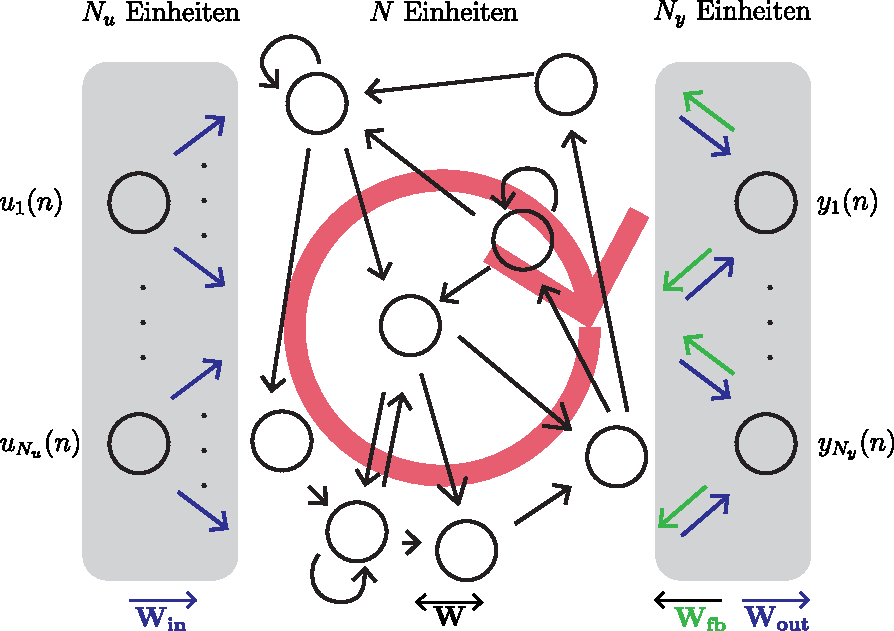
\includegraphics[width = 0.7 \textwidth]{figures/illustrations/esn_structure.pdf}
    \caption{Schematische Darstellung eines \textsc{ESN}. Von links nach rechts durchläuft das Eingangssignal $u(n)$ erst $N_u$ Eingangseinheiten, danach ein Reservoir mit $N$ Einheiten, bis schließlich die Ausgabe $y(n)$ mittels $N_y$ Ausgabeeinheiten gebildet wird. (nach \citep{jeagerTut2002, Ma2013}).}
    \label{fig:esn_structure}
\end{figure}


Anhand der inneren Zustände lassen sich nun noch die sogenannten erweiterten inneren Zustände $x(n) = [b_{out}; \vec{s}(n); \vec{u}(n)] \in \mathbb{R}^{1 + N_u + N}$ definieren, wobei $b_{out}$ ein \textit{Bias} für die Ausgabe darstellt. 

Aus diesen erweiterten inneren Zuständen kann nun die Ausgabe $\vec{y}(n)$ konstruiert werden. Dies kann entweder im Sinne einer Linearkombination durch die Ausgangsmatrix $\mathbf{W_{out}} \in \mathbb{R}^{(1 + N_u + N) \times N_y}$ oder durch andere nicht lineare Regressionsalgorithmen wie beispielsweise einer \textsc{Support Vector Machine (SVM)} durchgeführt werden. Im Folgenden wird nur der Fall einer Linearkombination betrachtet, da sich für die anderen Methoden ein analoges Verfahren ergibt.
In diesem Fall berechnet sich die Ausgabe mittels
\begin{align}
\vec{y}(n) = f_{out} \left( \mathbf{W_{out}} \vec{x}(n) = \mathbf{W_{out}} [b_{out}; \vec{s}(n); \vec{u}(n)] \right),
\end{align}
wobei $f_{out}$ die Transferfunktion der Ausgabe ist. Für diese kann in den meisten Fällen (so auch in dieser Arbeit) die Identität $f_{out}(x) = x$ genutzt werden.\\

Während die Matrix $\mathbf{W_{out}}$ durch den Trainingsvorgang bestimmt wird, werden die Matrizen $\mathbf{W_{in}}$ und $\mathbf{W}$ a priori generiert und festgelegt. Hierbei hat sich für das Generieren der Eingangsmatrix eine zufällige Anordnung von zufälligen Gleitkommazahlen zwischen $-0.5$ und $0.5$ als geschickt herausgestellt. Falls ein Feedback gewünscht ist, also Gleichung (\ref{eq:esn_stateeq_feedback}) genutzt wird, wird $\mathbf{W_{fb}}$ gleichartig konstruiert. Auf das Generieren der inneren Matrix $\mathbf{W}$ wird in Abschnitt \ref{sc:esn_theory} genauer eingegangen.

\subsection{Trainingsvorgang}
Nachdem der Aufbau des Netzwerkes beschrieben ist, ergibt sich nun die Frage, wie der Trainingsvorgang durchgeführt wird.

Hierfür wird für die Zeiten $n=0, ..., T_0$ das \textsc{ESN} mit dem Signal $\vec{u}(n)$ betrieben, wobei $T_0$ die \textit{transiente Zeit} beschreibt. Hierdurch soll das System aus seinem zufällig gewähltem Anfangszustand in einen charakteristischen Zustand übergehen. Anschließend wird das System für Zeiten $n < T$ weiter betrieben und die erweiterten Zustände $\vec{x}(n)$ als Spalten in der \textit{Zustandsmatrix} $\mathbf{X} \in \mathbb{R}^{(1 + N_u + N) \times T}$ gesammelt. Analog dazu werden die gewünschten Ausgaben $\vec{y}(n)$ nach dem Anwenden der Inversen $f^{-1}_{out}$ der Ausgabe-Transferfunktion $f_{out}$ auch als Spalten in der \textit{Ausgabematrix} $Y \in \mathbb{R}^{N_y \times T}$ gesammelt.
Nun wird eine Lösung der Gleichung
\begin{align}
\mathbf{Y} = \mathbf{W}_{out} \mathbf{X}
\end{align}
für $\mathbf{W}_{out}$ gesucht. Hierfür stehen mehrere Verfahren zur Verfügung, von denen zwei prominente erwähnt sein sollen.
Zum einen kann die Lösung durch eine \textit{Tikhonov Regularisierung} mittels der Regularisierung $\beta \cdot ||\vec{W}_{out, i}||^2$ der Gewichtsmatrix mit der Konstante $\beta$ erhalten werden. Hierbei steht $\vec{W}_{out, i}$ für die jeweils $i$-te Zeile der Gewichtsmatrix. Das Verfahren
\begin{align}
\label{eq:tikhonov}
\mathbf{W}_{out} = \mathbf{Y} \mathbf{X}^T \left(\mathbf{X} \mathbf{X}^T + \beta I \right)^{-1}
\end{align}
ist sehr leistungsstark, aber auch teilweise numerisch instabil. Bei geeigneter Wahl von $\beta$ können die besten Ergebnisse hinsichtlich der Genauigkeit der Vorsage erzielt werden \cite{lukoseviciusa2009}. Deshalb wird in dieser Arbeit auch nur dieses Lösungsverfahren verwendet. Die weiteren Lösungsansätze für das Gleichungssystem sind nur aus Gründen der Vollständigkeit angegeben.\\

Zum anderen kann zur Lösung die \textit{Moore-Penrose-Pseudoinverse} $\mathbf{X}'$ genutzt werden, sodass für die Ausgabematrix
\begin{align}
\label{eq:pseudo_inverse}
\mathbf{W}_{out} = \mathbf{Y} \mathbf{X}'
\end{align}
folgt. Dieses Verfahren ist zwar sehr rechenaufwendig aber dafür numerisch stabil \cite{lukoseviciusa2009, jaeger2012}. Nichts desto trotz, kann allerdings auf Grund des Fehlens einer Regularisierung leicht der Effekt des \textsc{Overfittings} auftreten. Auf Grund dessen wird es in dieser Arbeit nicht verwendet.\\

Um den Effekt des Overfittings bei der Verwendung der Psuedoinversen zu reduzieren, kann in der Zustandsgleichung (\ref{eq:esn_stateeq}) beziehungsweise (\ref{eq:esn_stateeq_feedback}) eine leichte normalverteilte Störung $\vec{\nu}(n)$ der Größenordnung $\num{1e-1}$ bis $\num{1e-5}$ addiert wird. Falls die \textit{Tikhonov Regularisierung} zur Lösung verwendet wird, erhöht die Verwendung der zufälligen Störung die Stabilität der Vorhersage des System. Dieser Ansatz beruht auf Empirie, da eine mathematische Begründung hierfür noch nicht vollständig gelungen ist \citep{jaeger2010, lukoseviciusa2009}. Anschaulich lässt sich das Vorgehen dadurch motivieren, dass hierdurch künstliche Datenpunkte in der nähe der vorhandenen Trainingsdaten emuliert werden, und somit eine größere Vielfalt an Daten während der Trainingsphase beobachtet wird.\\

Zusammenfassend ergibt sich somit der folgende Funktionsablauf für die Anwendung eines \textsc{ESN}:

\singlespacing
\begin{enumerate}
	\item Zufälliges Generieren der Matrizen $\mathbf{W}_{in}, \mathbf{W}_{fb}$ und Konstruktion der Matrix $\mathbf{W}$ 
	\item Einspeisen des Signals $u(n)$ und Konstruktion der Zustandsmatrix $\mathbf{X}$ und der Ausgabematrix $\mathbf{Y}$ 
	\item Berechnung der Ausgabematrix $\mathbf{W}_{out}$
	\item Einspeisen des Signals $u(n)$ für Vorhersagen des Signales $y(n)$ für $n > T$
\end{enumerate}
\onehalfspacing

Zusätzlich zu diesen Eigenschaften wird die Dynamik des Reservoirs auch von dessen Größe $N$ bestimmt. Es kann gezeigt werden, dass die Gedächtnisleistung eines Reservoirs stark von dieser abhängt. Somit ist es ratsam für Aufgaben, die eine lange Gedächtnisleistung benötigen, ein großes und für Aufgaben, die nur ein Kurzzeitgedächtnis benötigten, ein kleines Reservoir zu benutzen \citep{jeagerTut2002}.





\subsection{Theoretischer Hintergrund}
\label{sc:esn_theory}
Um die mathematischen Eigenschaften beschreiben zu können, sind zuerst zwei Definitionen nötig \cite{yildiz}.

\begin{definition}[Kompatibler Zustand]
Sei $S : X \times U \rightarrow X$ ein \textsc{ESN} mit der Zustandsgleichung $\vec{x}_{n+1} = F \left( \vec{x}_n, \vec{u}_{n+1} \right)$. Eine Folge von Zuständen $(\vec{x}_n)_n$ ist kompatibel mit der Eingangsfolge $(\vec{u}_n)_n$, wenn $\vec{x}_{n+1} = F\left( \vec{x}_n, \vec{u}_{n+1} \right), \forall n \leq 0$ erfüllt ist.
\end{definition}

\begin{definition}[Echo State Eigenschaft (ESP)]
Ein \textsc{ESN} $S : X \times U \rightarrow X$ besitzt die \textit{Echo State Eigenschaft} genau dann wenn eine Nullfolge $(\delta_n)_{n \geq 0}$ existiert, sodass für alle Zustandsfolgen $(\vec{x}_n)_n, (\vec{x}'_n)_n$ die kompatibel mit der Eingangsfolge $(\vec{u}_n)_n$ sind gilt, dass $\forall n \geq 0 ||x_n - x'_n|| < \delta_n$
\end{definition} 
Dies bedeutet, dass nachdem das Netzwerk lang genug betrieben worden ist, der Zustand nicht mehr von dem beliebig gewähltem Anfangszustand abhängt. Diese Eigenschaft ist notwendig, damit das \textsc{ESN} Vorhersagen treffen kann \cite{jeagerTut2002}.\\

Nun stellt sich die Frage, wann ein Netzwerk diese Eigenschaft besitzt. Es wird schnell klar, dass dies hauptsächlich durch die Gewichtsmatrix $\mathbf{W}$ bestimmt wird. Betrachtet man die Zustandsgleichung des Netzwerkes, so lässt sich auf Grund des \textit{Banachschen Fixpunktsatzes} erkennen, dass die \textit{ESP} für alle Eingänge $\vec{u}_n$ vorliegt, sobald $||\vec{x}_{n+1} - \vec{x}'_{n+1}|| < ||\vec{x}_n - \vec{x}'_n||$ für zwei kompatible Zustände $\vec{x}_n \neq \vec{x}'_n$ erfüllt ist \cite{jaeger2010}.
Hieraus ergibt sich, dass die \textit{ESP} vorliegt, wenn 
\begin{align}
\label{eq:theory_old_requirement}
|1-\alpha(1-\sigma_{max}(\mathbf{W}))| < 1
\end{align}
erfüllt ist, wobei $\sigma_{max}(\mathbf{W})$ der größte Singulärwert ist \cite{jaeger2007}.\\
Weitergehend ist bekannt, dass für Systeme bei denen der Spektralradius $\rho(\mathbf{W}) > 1$ ist diese Eigenschaft nicht vorliegen kann, sofern $\vec{u}_n = 0$ möglich ist \cite{jaeger2007, jaeger2010}.\\

Hieraus ergab sich lange Zeit die falsche Annahme, dass für Systeme mit $\rho(\mathbf{W}) < 1$ die Eigenschaft stets garantiert ist. Wie allerdings gezeigt werden konnte, ist dies nicht der Fall \citep{yildiz}. Stattdessen konnte gezeigt werden, dass eine hinreichende Bedingung durch
\begin{align}
\label{eq:theory_sufficient_requirement}
\rho(\alpha |\mathbf{W}|+(1-\alpha) \mathbf{I}) < 1
\end{align}
gegeben ist - wobei als Betrag der Matrix hier das elementweise Betragsnehmen gemeint ist. Diese Bedingung ist weniger einschränkend als Gleichung (\ref{eq:theory_old_requirement}) \cite{yildiz}.\\

Weitergehend hat sich in Experimenten gezeigt, dass eine dünnbesetze Gewichtsmatrix $\mathbf{W}$ zu reicheren Dynamiken innerhalb des Reservoirs führen kann \citep{jaeger2010}. Eine solche dünnbesetze Matrix bedeutet, dass nicht mehr jedes Neuron mit jedem anderen Neuron verbunden ist, sondern dass nur noch ein relativer Anteil $\epsilon$ dieser Verbindungen vorhanden ist. Da durch eine größere Anzahl an verschiedenen internen Dynamiken vielfältigere Funktionen besser approximiert werden können, kann die Vorhersagequalität durch einen Geringen $\epsilon$ Wert erhöht werden.\\

Darauf basierend kann nun eine Methode nach \cite{yildiz} angegeben werden, um die Gewichtsmatrix $\mathbf{W}$ zu konstruieren:

\singlespacing
\begin{enumerate}
	\item Generiere zufällige Matrix $\mathbf{W}$ mit $\mathbf{|W|} = \mathbf{W}$ bei der in jeder Zeile nur $\epsilon$ Einträge ungleich $0$ sind.
	\item Skaliere $\mathbf{W}$, sodass Gleichung (\ref{eq:theory_sufficient_requirement}) erfüllt ist.
	\item Wechsel zufällig das Vorzeichen von ungefähr der Hälfte aller Einträge.
\end{enumerate}
\onehalfspacing

Statt dieser Vorschrift wurde zuvor oftmals $\mathbf{W}$ zufällig generiert und anschließend nur $\rho(\mathbf{W})$ statt $\rho(|\mathbf{W}|)$ skaliert, was mit unter zu instabilen Systemen geführt hat. Da allerdings auch für Systeme mit einem Spektralradius $ > 1$ die \textit{ESP} beobachtet werden kann für nicht verschwindende Eingänge $\vec{u}_n$, ist es ratsam auch effektive Spektralradien jenseits $1$ auszuprobieren.
\clearpage

\section{Anwendungen}
\label{chp:applications}
Um den Aufwand für die spätere Benutzung zu reduzieren, ist zuerst eine allgemeine Implementation des \textsc{ESN}s geschrieben worden, welche nun anhand zweier exemplarischer Systeme getastet worden ist.

\subsection{Vorhersage eines Rössler-Systems}
Eine erste Anwendung um die Möglichkeiten eines \textsc{ESN} zu demonstrieren besteht in der Vorhersage des Verhaltens eines \textit{Rössler-Systems}
\begin{align}
\label{eq:application_roessler_pde}
\begin{split}
\dot{x} &= -(y+z)\\
\dot{y} &= x + 0.25 \cdot  y\\
\dot{z} &= 0.4 + (x - 8.5)\cdot z.
\end{split}
\end{align}
Dieses System zeigt ein chaotisches Verhalten und stellt somit eine herausfordernde Aufgabe für die zeitliche Vorhersage dar.\\
Hierbei werden zwei verschiedene Aufgaben betrachtet:\textit{(a)} die Vorhersage von $x'(t) \approx x(t+5)$ durch die Kenntnis von $x(t)$ und \textit{(b)} die Kreuz-Vorhersage $y(t)$ durch $x(t)$. Für beide Aufgaben wurde das System für jeweils $6000$ Schritte mit einer Abtastrate $\Delta t = 0.1$ in Analogie zu \cite{parlitz2005} simuliert, wobei die Hälfte der Daten für das Training und der Rest für die Testergebnisse verwendet worden ist.

\subsubsection[Vorhersage $x(t) \rightarrow x(t+5)$]{Vorhersage $\pmb{x(t) \rightarrow x(t+5)}$}
Für diese erste Aufgabe ist durch eine \textsc{GridSearch} ein geeignetes System gefunden werden, dessen Parameter in der Tabelle \ref{tab:application_roessler} dargestellt sind. Dafür wurde ein größerer Bereich des Hyperparameterraumes systematisch abgetastet und die jeweilige Leistung des sich ergebenen \textsc{ESN}s ermittelt, um anschließend die bestmöglichen Parameter zu wählen. Als Maß für diese Optimierung wurde der \textit{Mean Square Error (MSE)}
\begin{align}
MSE = \sum_n \left(x(t+5) - x'(t) \right)^2
\end{align}
zwischen der Vorhersage $x'(t)$ und dem tatsächlichem Wert $x(t+5)$ benutzt.

\begin{table}[H]
	\centering
	\captionsetup{width=0.9\linewidth}
		\begin{tabular}{|c|c|c|}
		\rule[-1ex]{0pt}{3.5ex} Variable & \hspace{4ex} Wert für \textit{(a)} \rule[-1ex]{4ex}{0pt} & \hspace{4ex} Wert für \textit{(b)} \rule[-1ex]{4ex}{0pt}\\ 
		\hline \hline 
		\rule[-1ex]{0pt}{3.5ex} $N$ & $300$ & $500$ \\ 
		\hline 
		\rule[-1ex]{0pt}{3.5ex} $\alpha$ & $0.25$ & $0.20$ \\ 
		\hline 
		\rule[-1ex]{0pt}{3.5ex} $\rho(|\mathbf{W}|)$ & $0.80$ & $0.70$\\ 
		\hline 
		\rule[-1ex]{0pt}{3.5ex} $\nu_{max}$ & $0.01$ & $0.01$\\ 
		\hline 
		\rule[-1ex]{0pt}{3.5ex} $\beta$ & $\num{1e-6}$ & $-$\\ 
		\hline 
	\end{tabular} 
	\caption{Auflistung der Parameter für das jeweilige \textsc{ESN} für (a) und (b).}
	\label{tab:application_roessler}
\end{table}

Der Trainingsvorgang wurde mittels der \textit{Tikhonov Regularisierung} nach Gleichung \ref{eq:tikhonov} durchgeführt. Im Training konnte ein Fehler von $MSE = 0.555 	$ erreicht werden, wobei sich im Testvorgang der Fehler zu $MSE = 0.237$ ergeben hat. Ein graphischer Vergleich zwischen dem Signal $y(t)$ und der Vorhersage $v(n)$ ist in Abbildung \ref{fig:application_roessler_a} zu finden.

\vspace{-3.75ex}
\begin{figure}[H]
    \centering
    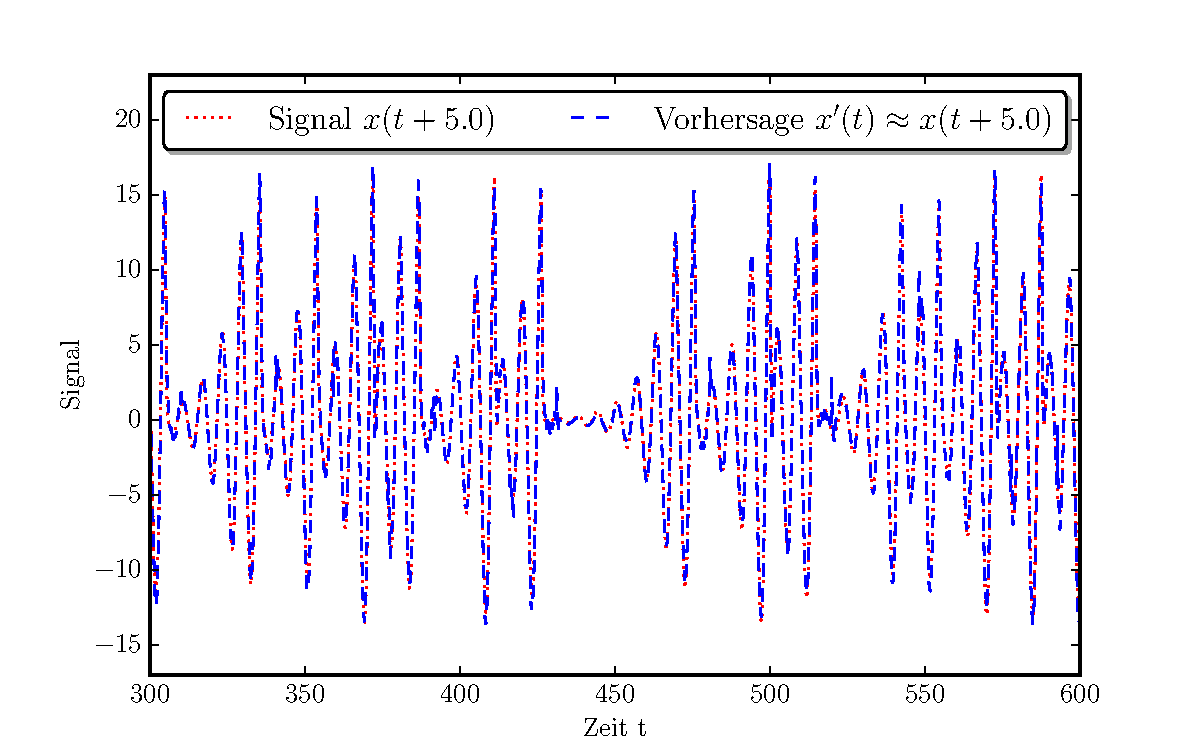
\includegraphics[width = 0.9 \textwidth]{figures/roessler_pred50.pdf}
    \caption{Darstellung des Signals $x(t+5.0)$ und der Vorhersage $x'(t) \approx x(t+5.0)$.}
    \label{fig:application_roessler_a}
\end{figure}



\subsubsection[Kreuz-Vorhersage $x(n) \rightarrow y(n)$]{Kreuz-Vorhersage $\pmb{x(n) \rightarrow y(n)}$}
Auch hierfür konnte sehr schnell durch eine \textsc{GridSearch} ein geeignetes System gefunden werden. Als Maß wurde ebenfalls der \textit{MSE} benutzt. Die gefundenen Parameter sind ebenso in der Tabelle \ref{tab:application_roessler} dargestellt.\\
Für das Auslesen wurde eine Linearkombination genutzt, wobei die Lösung $\mathbf{W}_{out}$ mittels der Pseudoinversen nach Gleichung \ref{eq:pseudo_inverse} bestimmt worden ist.\\

Damit wurde für den Trainingsvorgang ein Fehler $MSE_{train} = 0.0025$ und für den Testvorgang von $MSE_{test} = 0.0001$ bestimmt. Die Darstellung der Vorhersage $y'(t)$ und des ermittelten Fehlers sind in den Abbildungen \ref{fig:application_roessler_b1} und \ref{fig:application_roessler_b2} zu finden.

\begin{figure}[H]
    \centering
     %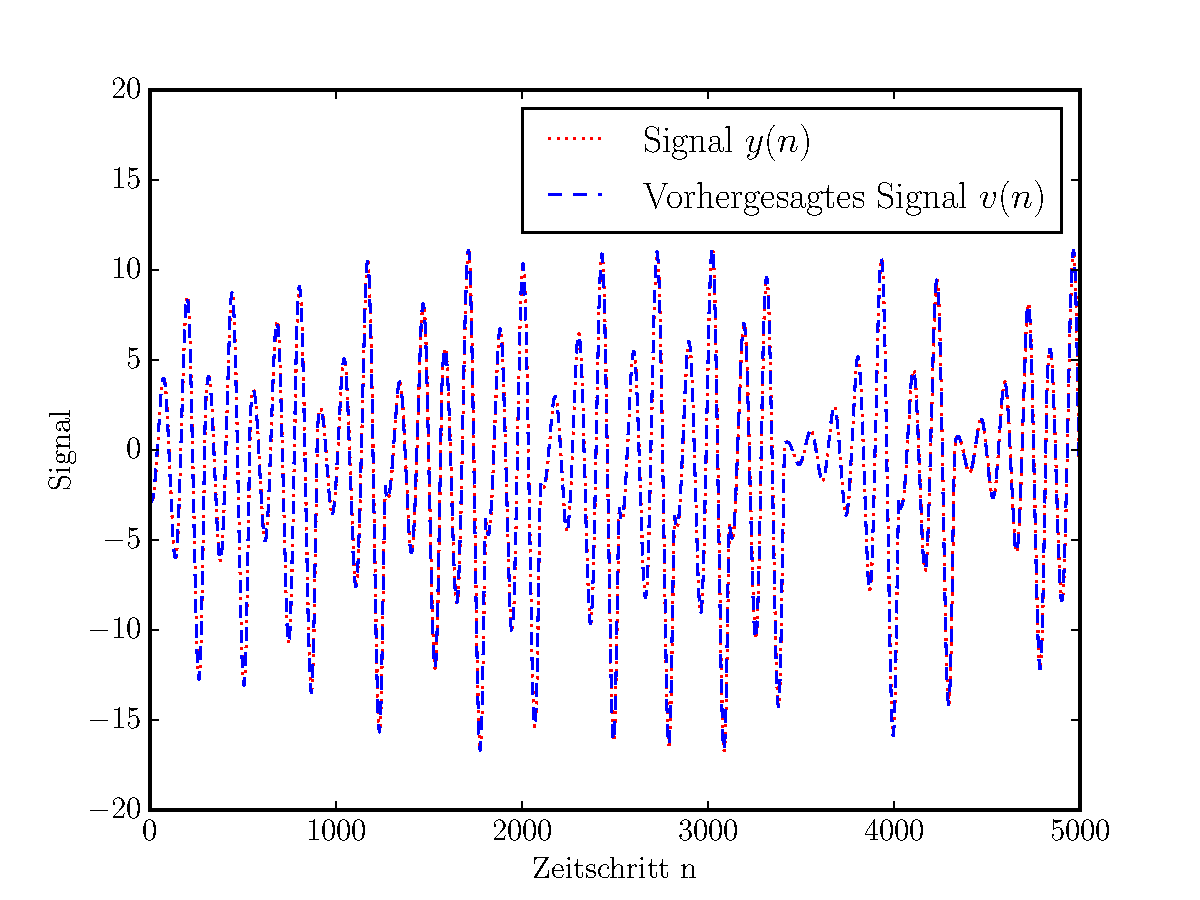
\includegraphics[width = 0.9 \textwidth]{figures/roessler_cross_pred.pdf}
     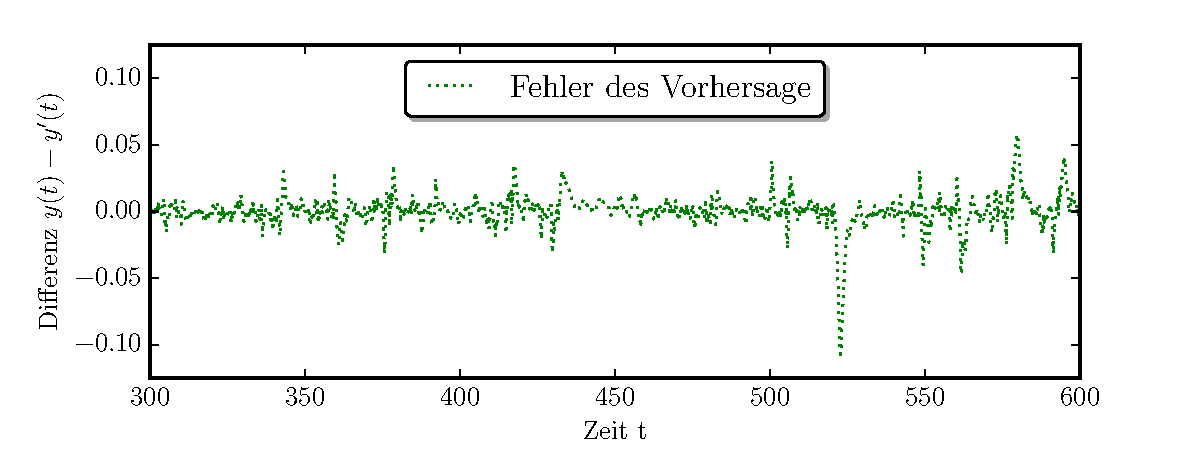
\includegraphics[width = 0.9 \textwidth]{figures/roessler_cross_err.pdf}
    \caption{Darstellung des Fehlers $y(t)-y'(t)$ zwischen dem Signal $y(t)$ und der Vorhersage $y'(t)$.}
    \label{fig:application_roessler_b1}
\end{figure}
 Im Vergleich zu anderen Publikationen \cite{parlitz2005} ergibt sich ein ähnlicher Fehler. Leider können hierbei nur die Graphen verglichen werden, da keine expliziten Fehler angegeben sind.


\begin{figure}[H]
    \centering
     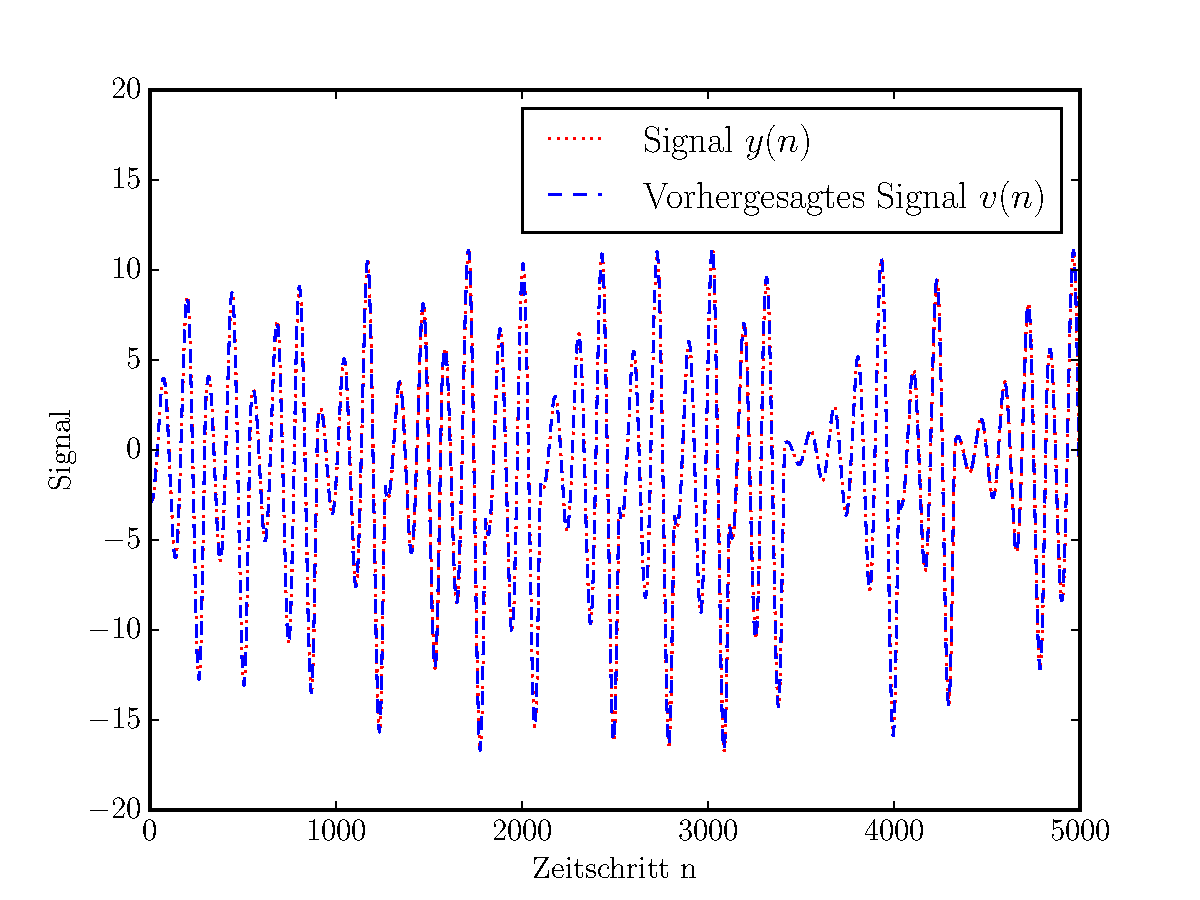
\includegraphics[width = 0.9 \textwidth]{figures/roessler_cross_pred.pdf}
      \caption{Darstellung des Signals $y(t)$ und der Vorhersage $y'(t)$.}
    \label{fig:application_roessler_b2}
\end{figure}

\clearpage

\subsection{Vorhersage eines Mackey-Glass-Systems}
\label{sec:mackey_glass}
Als nächste Anwendung wird ein \textit{Mackey-Glass-System}
\begin{align}
\label{eq:application_mackey_glass_pde}
\begin{split}
\dot{x}(t) &= \beta \frac{x(t-\tau)}{1+x(t-\tau)^n}-\gamma x(t)\\
\end{split}
\end{align}
betrachtet, wobei $\tau = 17, n=10, \gamma=0.1, \beta = 0.2$ gewählt wurden. Dies ist eine beliebte Aufgabe im Bereich der Vorhersagen chaotischer Zeitreihen.\\
Für dieses System wurde in Analogie zu  \citep{caraballo2014} die Vorhersage $x(t) \rightarrow x(t+84)$ betrachtet, wobei die Parameter aus Tabelle \ref{tab:application_mackeyglass} genutzt wurden. Mittels der expliziten \textit{Euler-Diskretisierung} 

\begin{align}
x(t+1) = x(t) + \Delta_t \cdot \left(\beta \frac{x(t-\tau)}{1+x(t-\tau)^n}-\gamma x(t)  \right)
\end{align}

sind Werte für $0 \leq t \leq 4000$ simuliert worden, wobei $\Delta_t=\num{1e-2}$ die zeitliche Diskretisierungskonstante ist. Nun sind die ersten $2000$ Werte für den Trainings und die anderen für den Test-Vorgang genutzt worden. Es wurde zur Lösung erneut die \textit{Tikhonov Regularisierung} nach Gleichung \ref{eq:tikhonov} benutzt.

\begin{table}[H]
	\centering
		\begin{tabular}{|c|c|}
		\rule[-1ex]{0pt}{3.5ex} Variable & \hspace{4ex} Wert \rule[-1ex]{4ex}{0pt}\\ 
		\hline \hline 
		\rule[-1ex]{0pt}{3.5ex} $N$ & $1000$ \\ 
		\hline 
		\rule[-1ex]{0pt}{3.5ex} $\alpha$ & $0.20$ \\ 
		\hline 
		\rule[-1ex]{0pt}{3.5ex} $\rho(\mathbf{W})$ & $1.25$ \\ 
		\hline 
		\rule[-1ex]{0pt}{3.5ex} $\nu_{max}$ & $\num{1e-4}$ \\ 
		\hline 
		\rule[-1ex]{0pt}{3.5ex} $\beta$ & $\num{1e-8}$ \\ 
		\hline 
	\end{tabular} 
	\caption{Auflistung der benutzten Parameter des \textsc{ESN}.}
\label{tab:application_mackeyglass}
\end{table}

Interessant ist, dass der Spektralradius größer $1.0$ ist. Dies widerspricht nicht direkt den Aussagen aus Abschnitt \ref{sc:theory}, da diese nur für Signale getroffen werden konnten, welche auch null sein können. Um dies auszuschließen ist ein konstanter \textit{Bias} von $1.0$ als weiteres Eingangssignal genutzt worden.\\
Eine Darstellung der Ergebnisse ist in Abbildung \ref{fig:application_mackeyglass} zu sehen. Der \textit{MSE} wurde für die Trainingsphase als $MSE_{train} = 0.0042$ und für die Testphase als $MSE_{test} = \num{9e-5}$ bestimmt.

\begin{figure}[H]
    \centering
    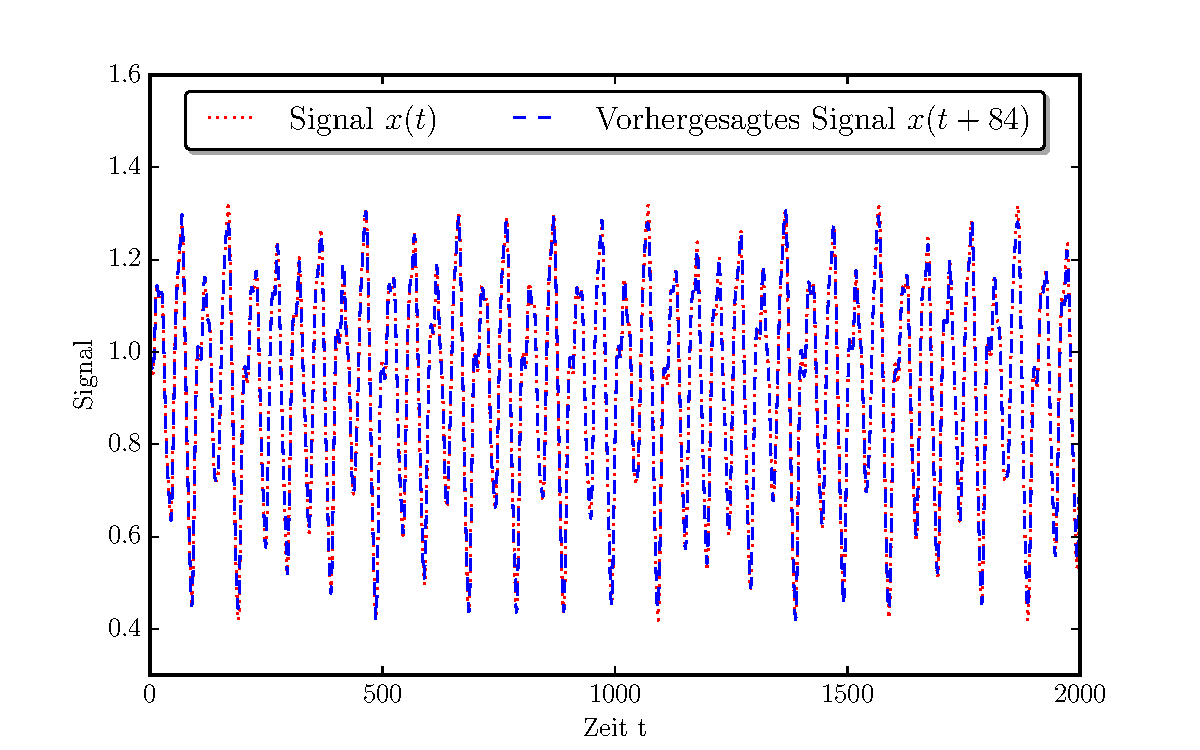
\includegraphics[width = 0.9 \textwidth]{figures/mackeyglass_pred.pdf}
    \caption{Darstellung des Signals $x(t)$ und der Vorhersage $x(t+84)$.}
    \label{fig:application_mackeyglass}
\end{figure}

Dies ist eine starke Verbesserung im Vergleich zu dem besten Ergebnis aus \citep{caraballo2014} mit $MSE = 0.0014$, wobei anzumerken ist, dass dort eine kleinere Trainings- und Testphase gewählt worden ist.
\clearpage

\chapter{Fazit}
In dieser Arbeit ist die Anwendung von \textit{Echo State Networks} für die Vorhersage von raumzeitlichen Dynamiken erregbarer Systeme untersucht worden. Dies ist anhand des \textit{Barkley}- und des \textit{Mitchell-Schaeffer}-Modells durchgeführt worden. Für die Vorhersage dieser raumzeitlichen Dynamiken ist ein sogenannter \textit{Messsonendenansatz} entwickelt und verwendet worden, bei dem nur lokal benachbarte Informationen für die Vorhersage genutzt werden.\\

Um die experimentellen Ergebnisse des \textsc{ESN}s einzuordnen, sind sie mit den Ergebnissen eines \textit{nächsten Nachbar}-Ansatzes und \textit{radialer Basisfunktionen} verglichen worden. Dabei sind Anwendungsarten betrachtet worden, welche für die Untersuchung von Herzen relevant sind: Zuerst ist eine nicht gemessene aus einer gemessenen Systemvariable bestimmt worden. Anschließend ist die elektrische Erregung auf der Herzoberfläche anhand des Fernfelds einer Elektrodenmessung rekonstruiert worden. Abschließend ist versucht worden die elektrische Erregung für unbekannte Regionen aus der Kenntnis weniger Randwerte vorzunehmen.\\

Es halt sich allgemein gezeigt, dass durch die Verwendung der \textit{Echo State Networks} in jedem Anwendungsbereich eine größere Genauigkeit erzielt werden konnte. Die \textsc{ESN}s stellen eine gut geeignete Methode zur Untersuchung und Vorhersage raumzeitlicher Dynamiken erregbarer Medien dar. Diese Erkenntnis passt zu den neusten wissenschaftlichen Publikationen auf dem Bereich \citep{Lu2017}.\\

Im Detail konnte die Kreuz-Prädiktion zwischen den zwei Systemvariablen nahezu fehlerfrei gelöst werden. Die Rekonstruktion der elektrischen Erregung konnte zudem die makroskopische Struktur der Dynamik rekonstruiert werden, aber nicht die Detailstruktur. Die Vorhersage des unbekannten Bereiches durch die Randwerte konnte nicht zufriedenstellend gelöst werden. Bereits für geringe Größen des vorherzusagenden Bereichs stieg der Fehler sowohl bei dem \textsc{ESN} als auch bei den Referenzmethoden sehr stark an. Dies kann ein Hinweis auf eine generelle physikalische Beschränktheit solcher Voraussagen sein. Es empfiehlt sich dieses Phänomen weitergehend zu untersuchen. \\

Es hat sich zudem herausgestellt, dass die Gewichtsmatrix $\mathbf{W_{out}}$ für verschiedene Bildpunkte eine große Ähnlichkeit aufzeigt. Somit bietet es sich an dieses Verhalten weiter zu untersuchen. Durch die Verwendung einer einzigen Auslesematrix lässt sich die Geschwindigkeit des \textsc{ESN} stark erhöhen. Zusätzlich wäre auch ein Einsatz anderer Methode aus dem Bereich des \textit{Machine Learnings} als Ersatz für die Auslesematrix, wie beispielsweise \textsc{FFNN}s denkbar.  
\clearpage

\section{Ausblick}
Für das Schreiben dieses Berichts hat sich die Wahl der \textsc{LaTeX}-Umgebung als gut geeignet herausgestellt. Die optische Darstellung von mathematischen Ausdrücken sowie des erklärenden Textes ist hierbei intuitiver umzusetzen als bei den bekannten Alternativen. Hierbei wurde die verwendete Literatur über \textsc{Zotero} und \textsc{BibTeX} direkt in den \textsc{LaTeX}-Quellcode eingebunden und zitiert.\\
Für die Literaturrecherche ist der Dienst \textsc{Google Scholar} benutzt worden, welcher eine umfassende Datenbank besitzt.\\

Das Programmieren der Anwendungsbeispiele wurde mit der Sprache \textsc{Python} und den bekannten Frameworks \textsc{Numpy} und \textsc{Scipy} umgesetzt. Diese Entscheidung wurde hauptsächlich durch die große Flexibilität dieser Sprache und der ausreichenden Leistung der Bibliotheken beeinflusst. Die hierbei entstandenen Grafiken wurden mit der \textsc{Pyplot} Bibliothek umgesetzt.\\ 

Dieses gesamte Vorgehen hat sich im Laufe des Praktikums als gut erwiesen und wird somit auch in der anschließenden Bachelorarbeit weiterverfolgt werden.
\clearpage

\nocite{*}

%\appendix

\clearpage
%% Bibliographie. Das Argument muss der Name der BIBTeX-Datenbank stehen.
%% Ein Beispiel fuer eine solche Datenbank finden Sie in bthesis_datenbank.bib
\bibliography{review_datenbank} 

%\chapter*{Danksagung}

%% Dieser Befehl MUSS am Ende stehen und erzeugt die Erklaerung ueber die
%% benutzten Mittel
%\Declaration

\end{document}